\Chapter{Appendices for Chapter~\ref{chap:chapter4}}

\section{Event displays}

%\begin{figure}[htb]
%\begin{center}
%\includegraphics[width=0.8\textwidth,angle=0]{figs/event-display/pteven2-177074_1171400298_711_3DTower.pdf}
%\includegraphics[width=0.8\textwidth,angle=0]{figs/event-display/pteven2-177074_1171400298_711_Lego.pdf}
%\end{center}
%\caption{Event display of a nicely balanced double W/Z-tagged event with a dijet invariant mass of 1.043~\TeVcc .
%The transverse momenta of the two leading jets are 0.538~\TeVcc and 0.476~\TeVcc .
%The invariant mass of the two leading pruned CA8 jets is 94.41 \GeVcc and 80.75 \GeVcc .
%}
%\label{fig:eventdisplay1}
%\end{figure}

\begin{figure}[htb]
\begin{center}
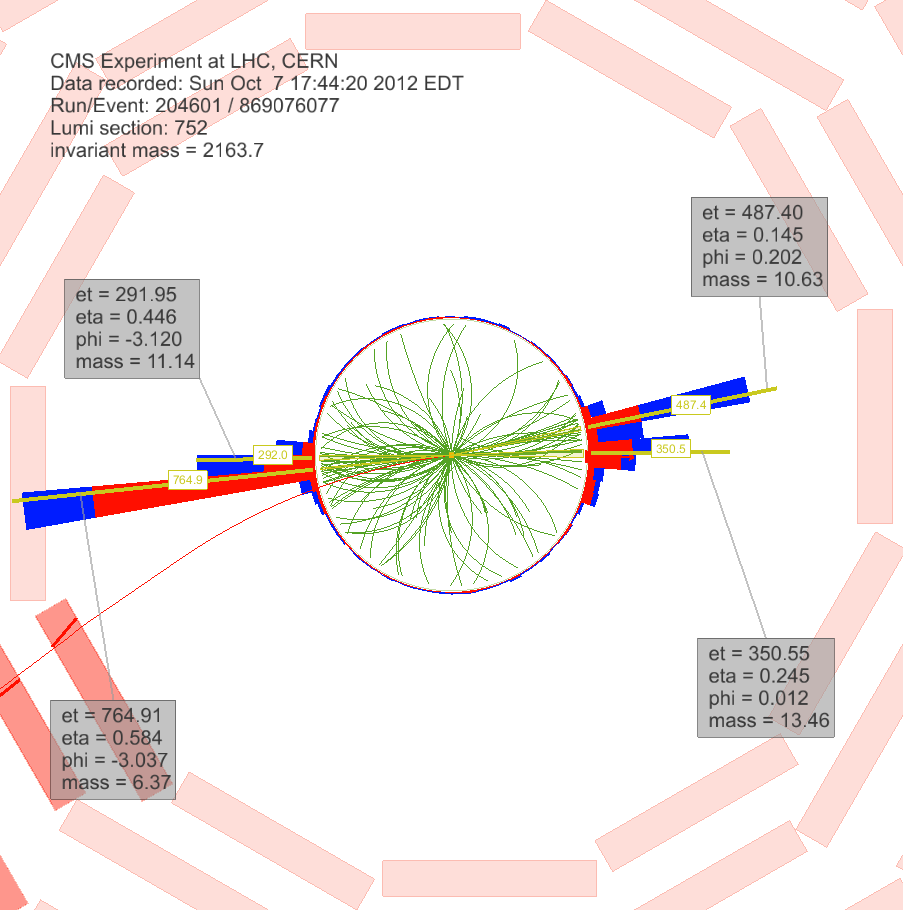
\includegraphics[width=0.6\textwidth,angle=0]{EXO-14-009/figs/event-display/highdoublemass/rho-phi-white.png}
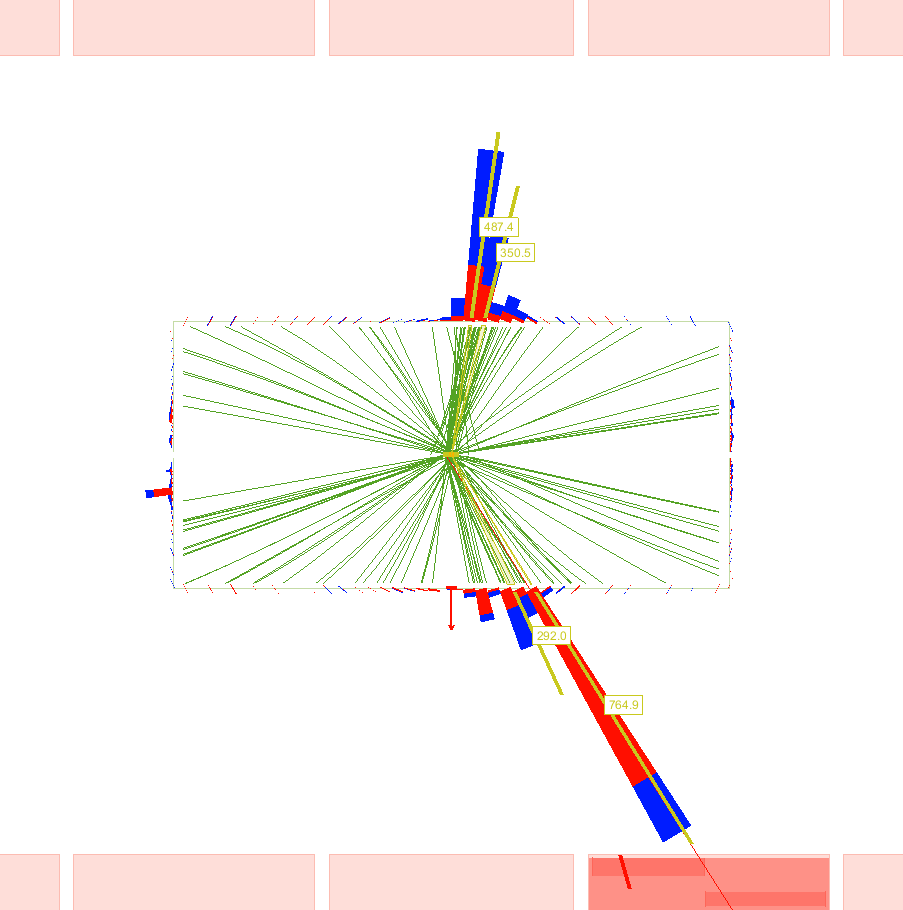
\includegraphics[width=0.6\textwidth,angle=0]{EXO-14-009/figs/event-display/highdoublemass/rho-z-white.png}
\end{center}
\caption{Event display of double W/Z-tagged event with the highest dijet invariant mass of 2.16~\TeVcc .
The transverse momenta of the two leading jets are 1.1~\TeVcc and 0.92~\TeVcc .
The invariant mass of the two leading pruned CA8 jets is 97.82 \GeVcc and 85.08 \GeVcc .
}
\label{fig:eventdisplay1}
\end{figure}

\begin{figure}[htb]
\begin{center}
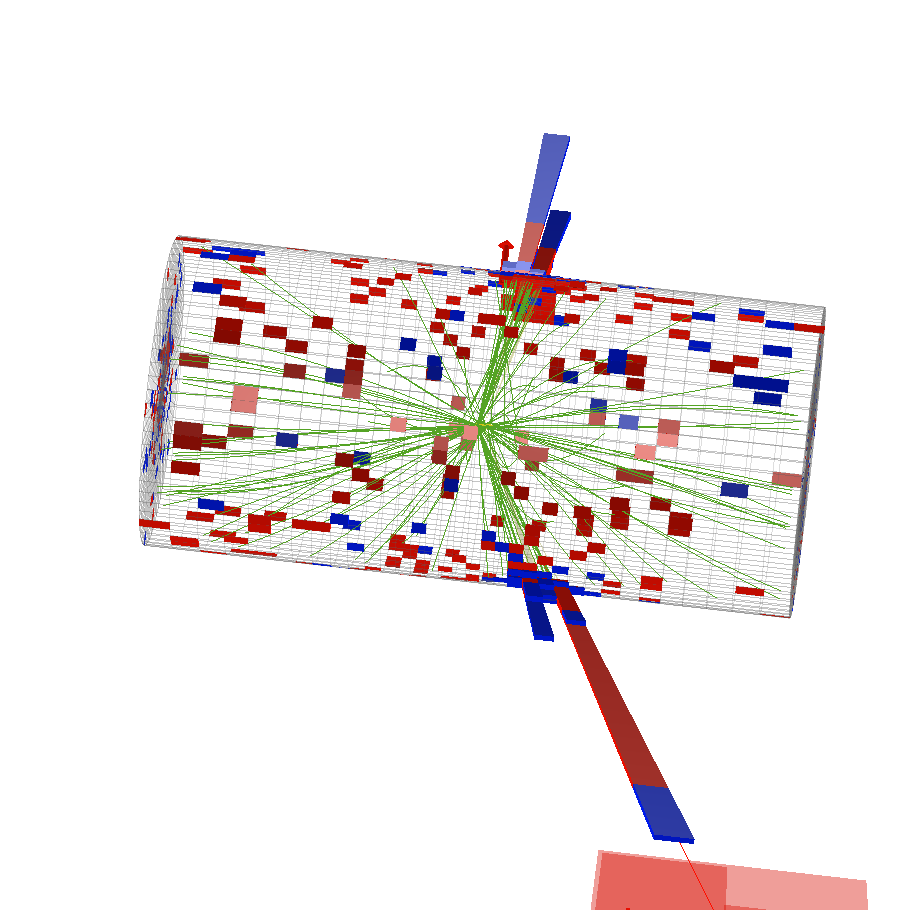
\includegraphics[width=0.6\textwidth,angle=0]{EXO-14-009/figs/event-display/highdoublemass/tower-white.png}
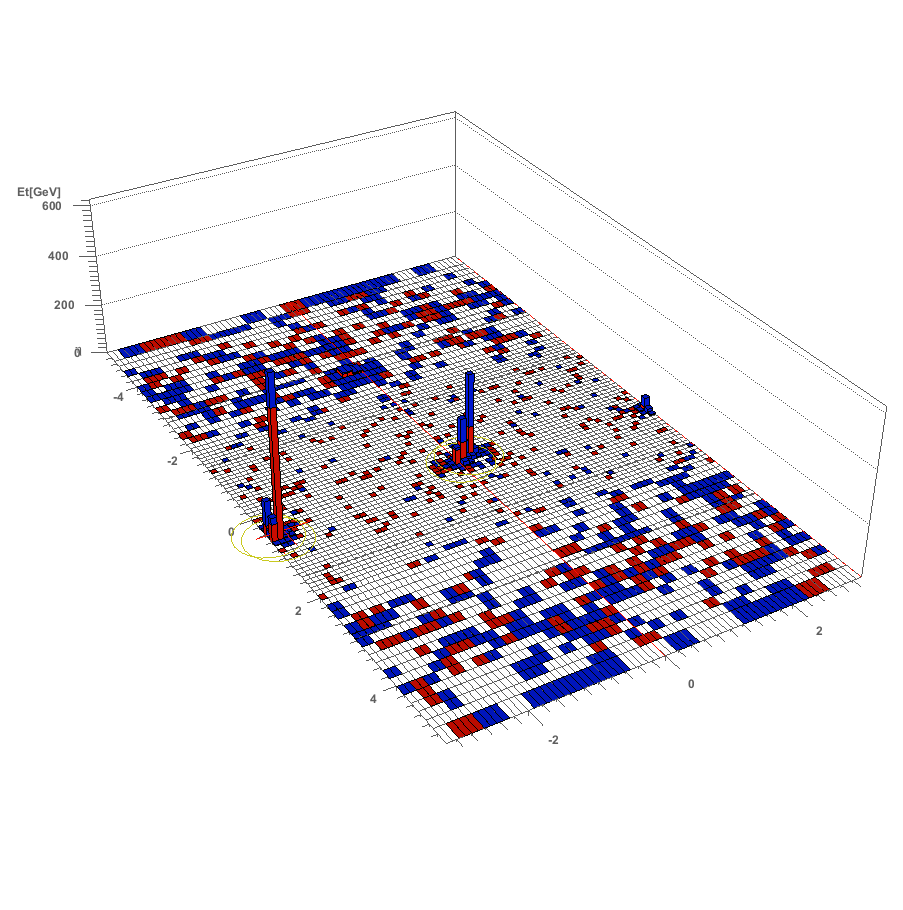
\includegraphics[width=0.6\textwidth,angle=0]{EXO-14-009/figs/event-display/highdoublemass/lego-white.png}
\end{center}
\caption{Event display of double W/Z-tagged event with the highest dijet invariant mass of 2.16~\TeVcc .
The transverse momenta of the two leading jets are 1.1~\TeVcc and 0.92~\TeVcc .
The invariant mass of the two leading pruned CA8 jets is 97.82 \GeVcc and 85.08 \GeVcc .
}
\label{fig:eventdisplay2}
\end{figure}

\begin{figure}[htb]
\begin{center}
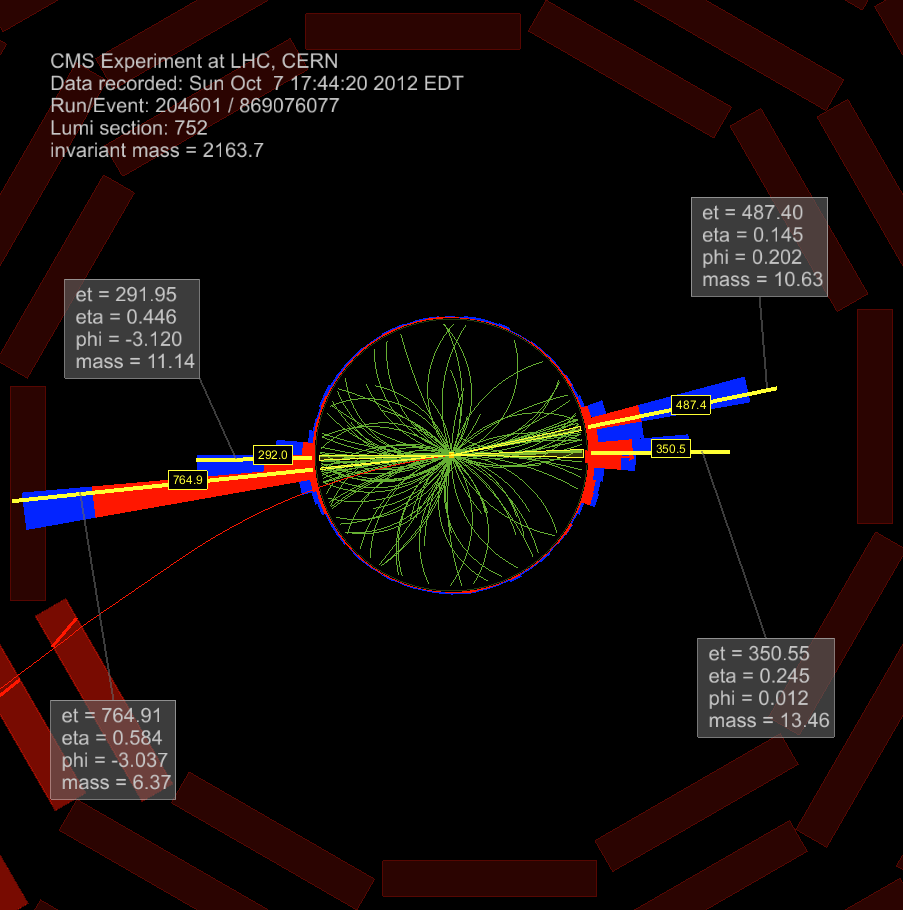
\includegraphics[width=0.6\textwidth,angle=0]{EXO-14-009/figs/event-display/highdoublemass/rho-phi-black.png}
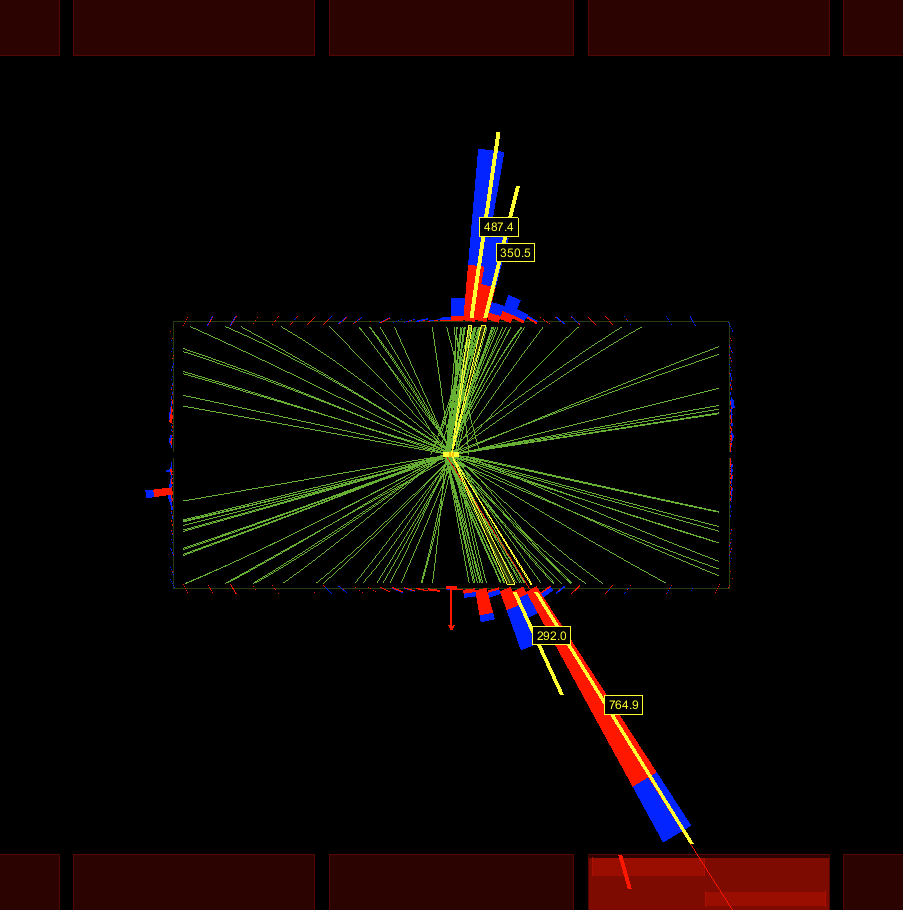
\includegraphics[width=0.6\textwidth,angle=0]{EXO-14-009/figs/event-display/highdoublemass/rho-z-black.png}
\end{center}
\caption{Event display of double W/Z-tagged event with the highest dijet invariant mass of 2.16~\TeVcc .
The transverse momenta of the two leading jets are 1.1~\TeVcc and 0.92~\TeVcc .
The invariant mass of the two leading pruned CA8 jets is 97.82 \GeVcc and 85.08 \GeVcc .
}
\label{fig:eventdisplay3}
\end{figure}

\begin{figure}[htb]
\begin{center}
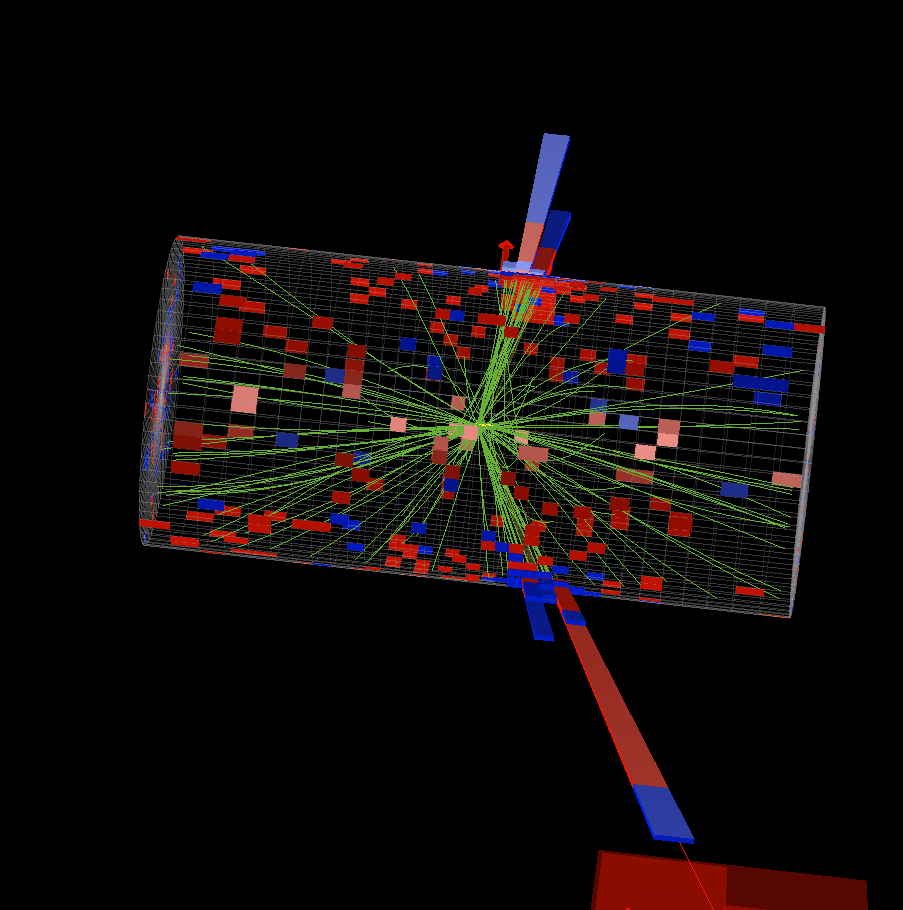
\includegraphics[width=0.6\textwidth,angle=0]{EXO-14-009/figs/event-display/highdoublemass/tower-black.png}
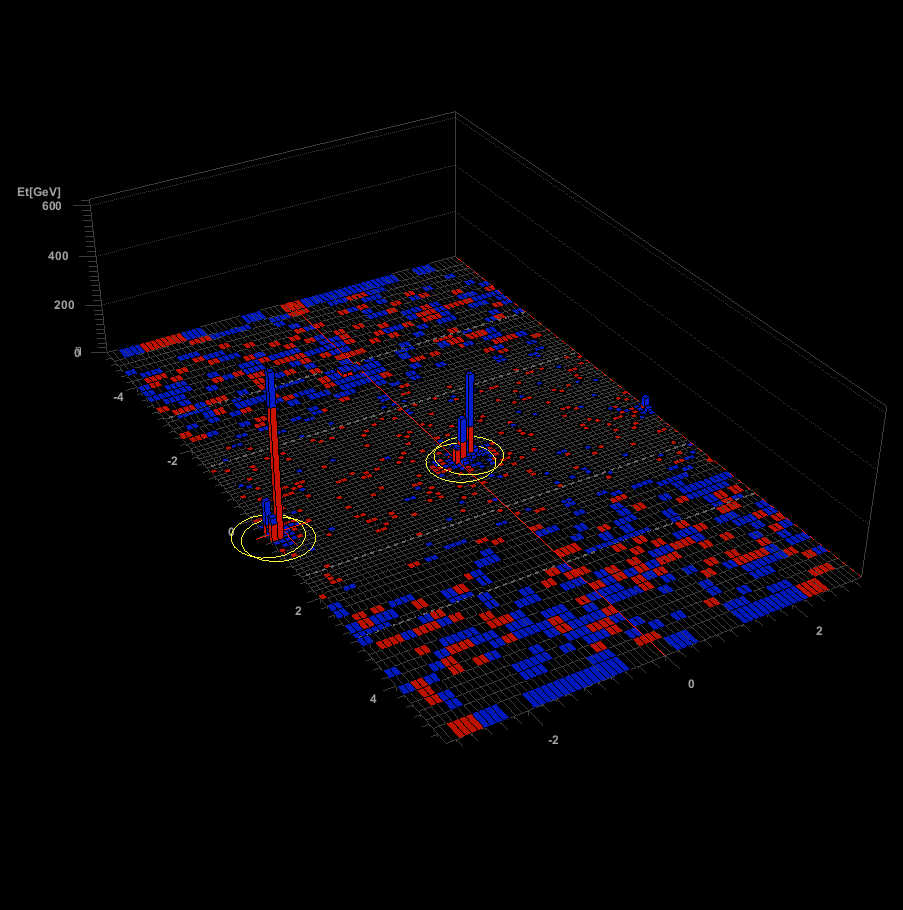
\includegraphics[width=0.6\textwidth,angle=0]{EXO-14-009/figs/event-display/highdoublemass/lego-black.png}
\end{center}
\caption{Event display of double W/Z-tagged event with the highest dijet invariant mass of 2.16~\TeVcc .
The transverse momenta of the two leading jets are 1.1~\TeVcc and 0.92~\TeVcc .
The invariant mass of the two leading pruned CA8 jets is 97.82 \GeVcc and 85.08 \GeVcc .
}
\label{fig:eventdisplay4}
\end{figure}

\begin{figure}[htb]
\begin{center}
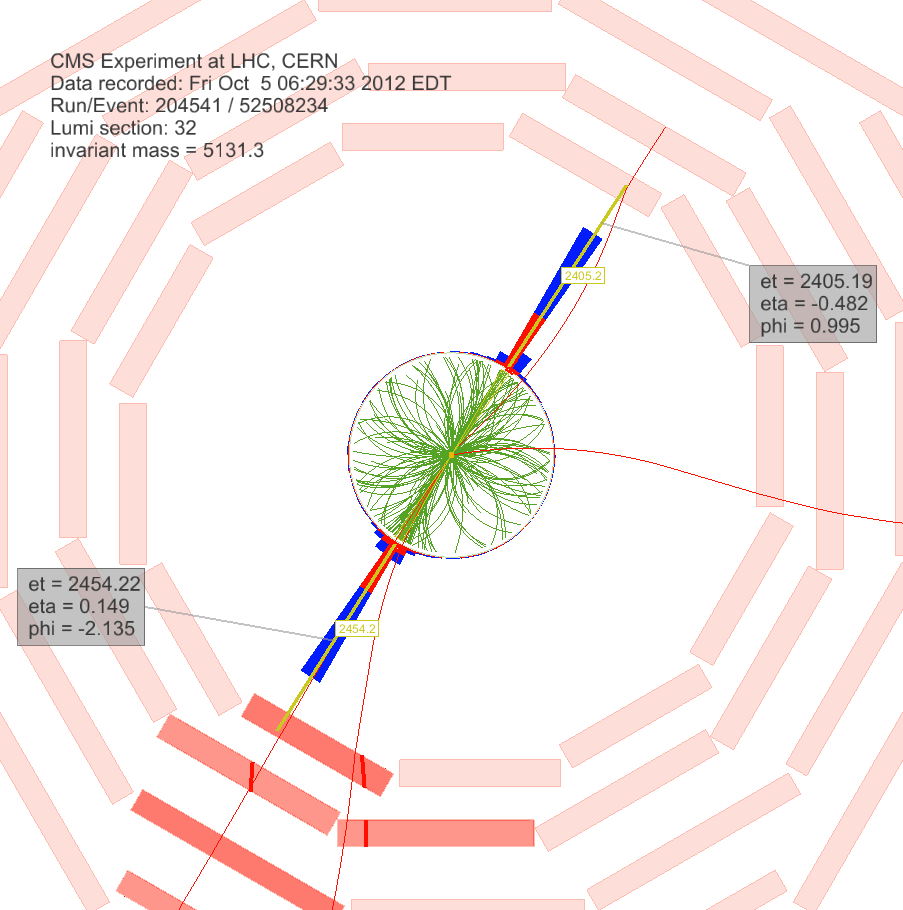
\includegraphics[width=0.6\textwidth,angle=0]{EXO-14-009/figs/event-display/prehighest/rho-phi-white.png}
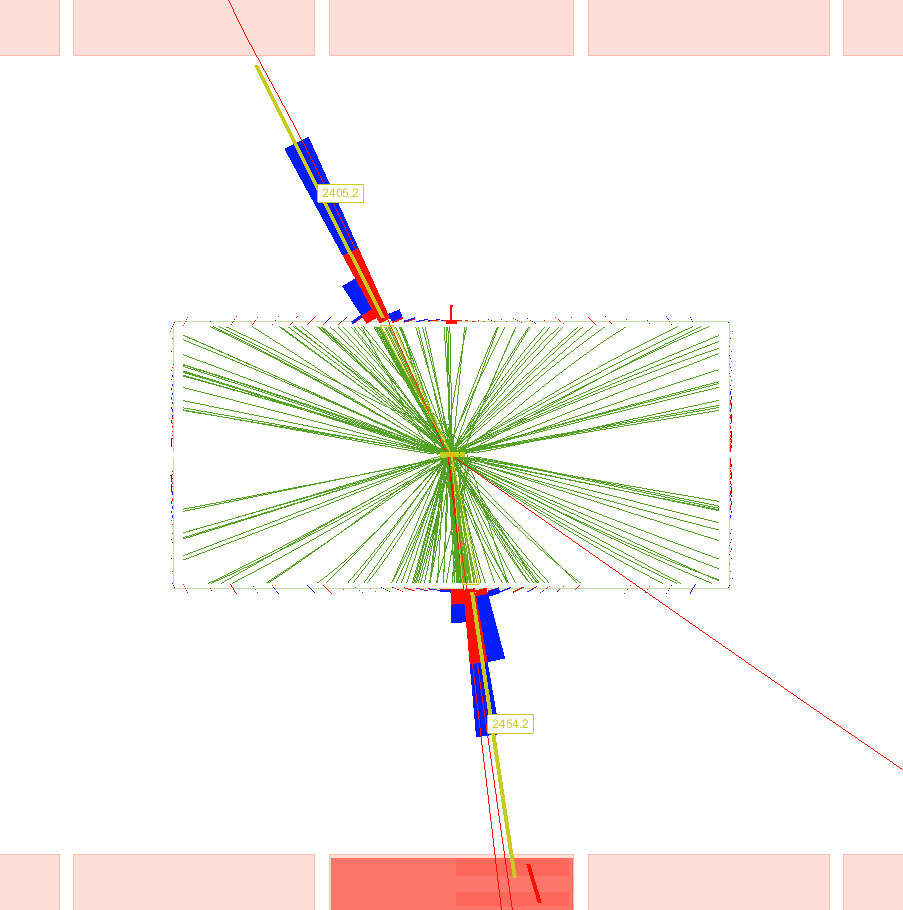
\includegraphics[width=0.6\textwidth,angle=0]{EXO-14-009/figs/event-display/prehighest/rho-z-white.png}
\end{center}
\caption{Event display of event with the highest dijet invariant mass of 5.13~\TeVcc .
The transverse momenta of the two leading AK5 jets are 2.45~\TeVcc and 2.40~\TeVcc .
}
\label{fig:eventdisplay11}
\end{figure}

\begin{figure}[htb]
\begin{center}
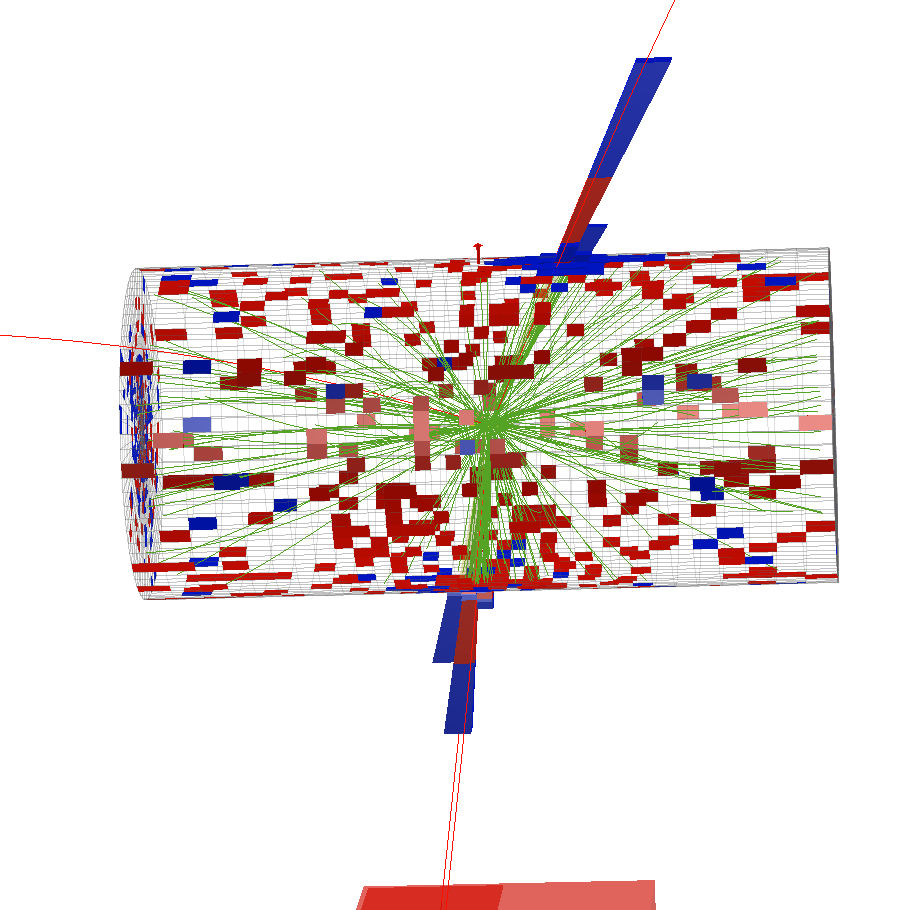
\includegraphics[width=0.6\textwidth,angle=0]{EXO-14-009/figs/event-display/prehighest/tower-white.png}
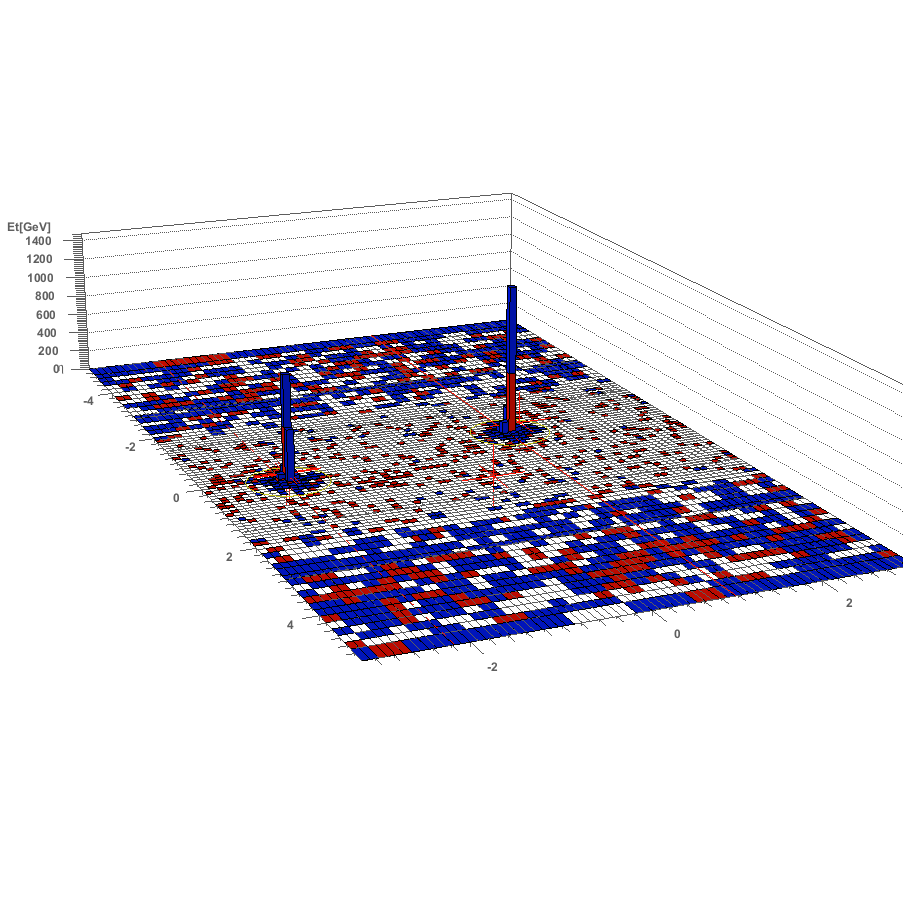
\includegraphics[width=0.6\textwidth,angle=0]{EXO-14-009/figs/event-display/prehighest/lego-white.png}
\end{center}
\caption{Event display of event with the highest dijet invariant mass of 5.13~\TeVcc .
The transverse momenta of the two leading AK5 jets are 2.45~\TeVcc and 2.40~\TeVcc .
}
\label{fig:eventdisplay12}
\end{figure}

\begin{figure}[htb]
\begin{center}
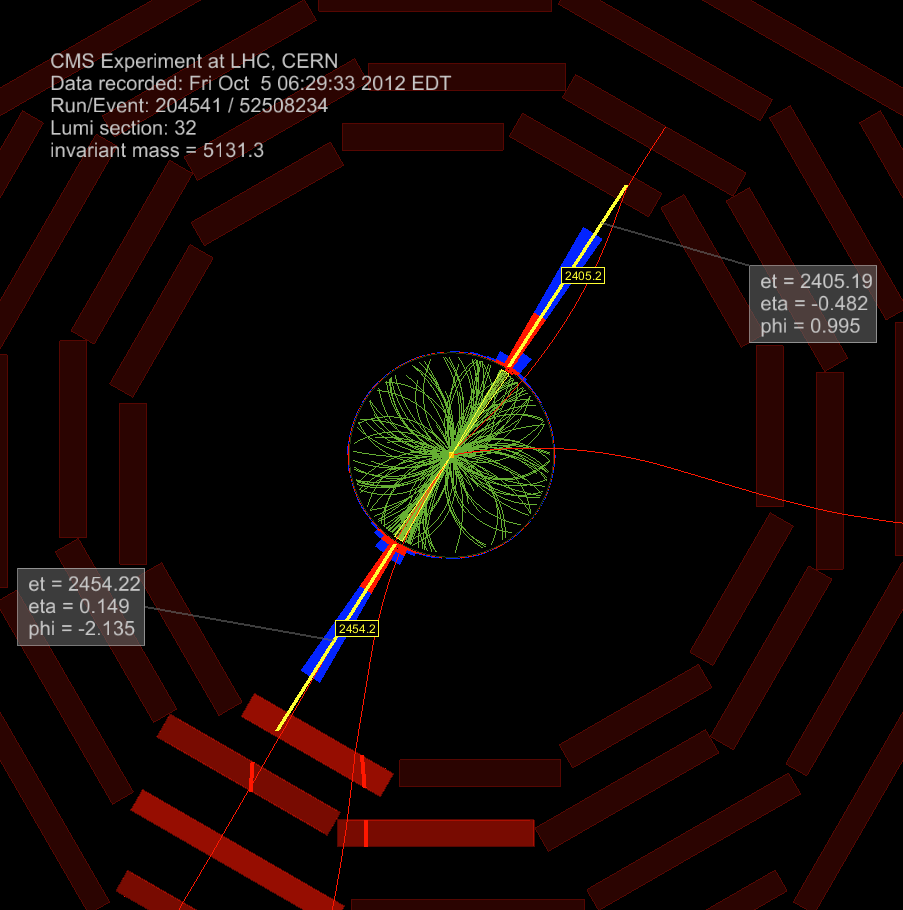
\includegraphics[width=0.6\textwidth,angle=0]{EXO-14-009/figs/event-display/prehighest/rho-phi-black.png}
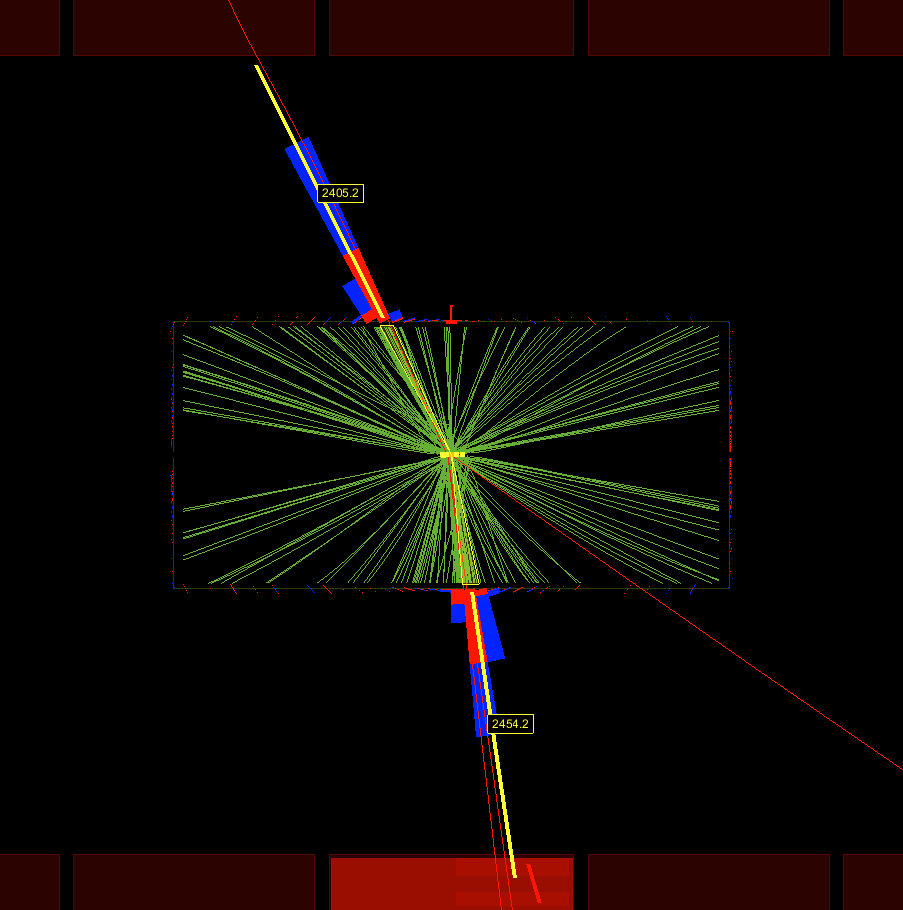
\includegraphics[width=0.6\textwidth,angle=0]{EXO-14-009/figs/event-display/prehighest/rho-z-black.png}
\end{center}
\caption{Event display of event with the highest dijet invariant mass of 5.13~\TeVcc .
The transverse momenta of the two leading AK5 jets are 2.45~\TeVcc and 2.40~\TeVcc .
}
\label{fig:eventdisplay13}
\end{figure}

\begin{figure}[htb]
\begin{center}
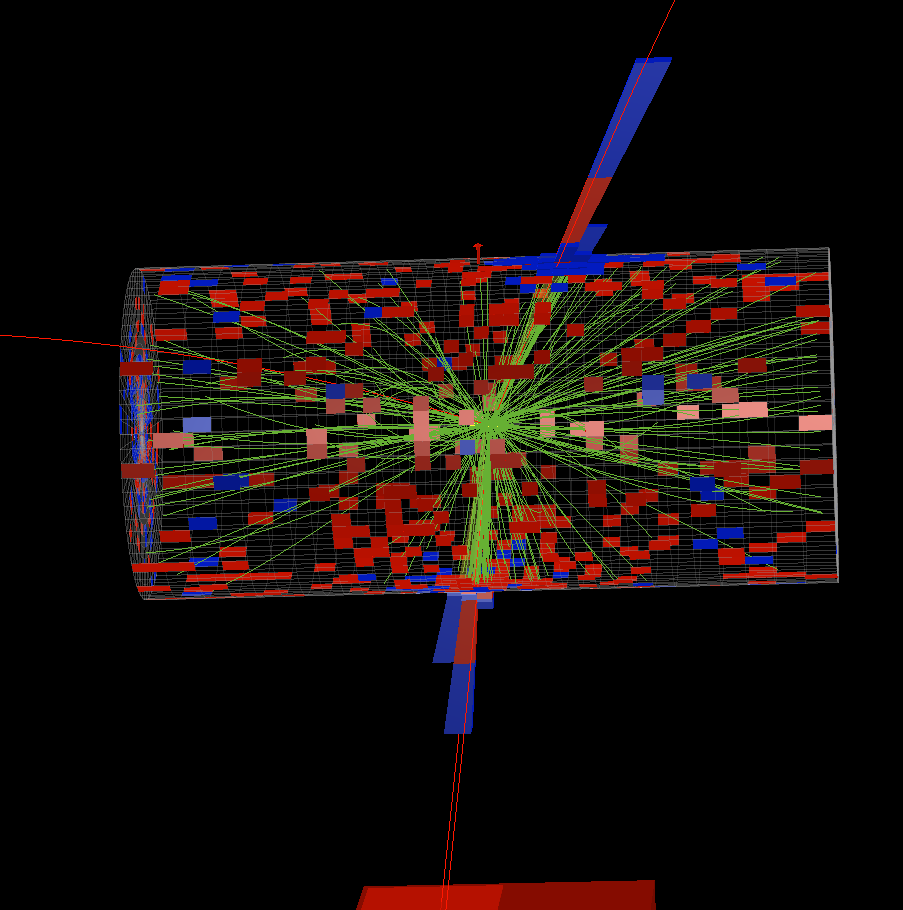
\includegraphics[width=0.6\textwidth,angle=0]{EXO-14-009/figs/event-display/prehighest/tower-black.png}
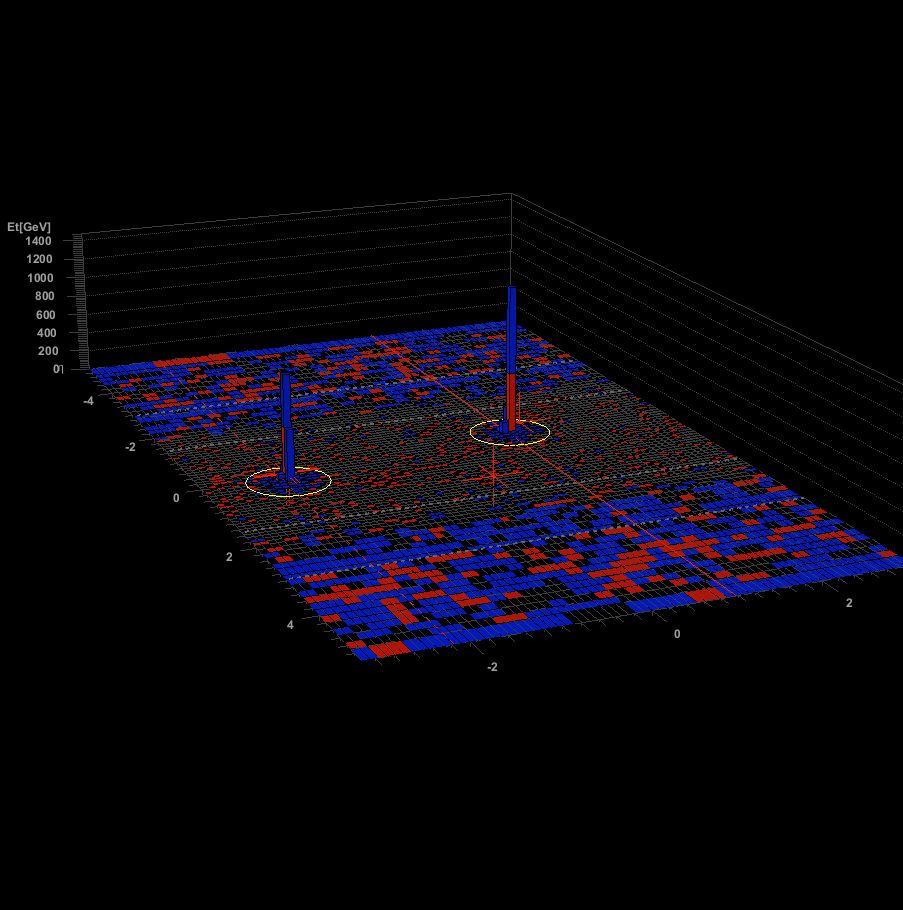
\includegraphics[width=0.6\textwidth,angle=0]{EXO-14-009/figs/event-display/prehighest/lego-black.png}
\end{center}
\caption{Event display of event with the highest dijet invariant mass of 5.13~\TeVcc .
The transverse momenta of the two leading AK5 jets are 2.45~\TeVcc and 2.40~\TeVcc .
}
\label{fig:eventdisplay14}
\end{figure}

\clearpage


